\documentclass[margin=5pt]{standalone}
\usepackage{tikz}
\usepackage{xcolor}

\definecolor{lightred}{RGB}{255,100,100}
\definecolor{lightblue}{RGB}{180,180,255}

\begin{document}
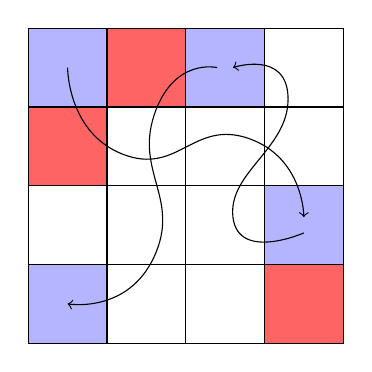
\begin{tikzpicture}
  \fill[lightred] (0, 2) rectangle (1, 3);
  \fill[lightred] (1, 3) rectangle (2, 4);
  \fill[lightred] (3, 0) rectangle (4, 1);
  \fill[lightblue] (0, 0) rectangle (1, 1);
  \fill[lightblue] (0, 3) rectangle (1, 4);
  \fill[lightblue] (3, 1) rectangle (4, 2);
  \fill[lightblue] (2, 3) rectangle (3, 4);

  \foreach \x in {0,1,2,3} {
    \foreach \y in {0,1,2,3} {
      \draw (\x, \y) rectangle (\x+1, \y+1);
    }
  }

  \draw[->] plot [smooth,tension=1.1] coordinates { (0.5, 3.5) (1.2, 2.4) (2.8, 2.6) (3.5, 1.6) };
  \draw[->] plot [smooth,tension=1.2] coordinates { (3.5, 1.4) (2.6, 1.6) (3.3, 3.1) (2.6, 3.5) };
  \draw[->] plot [smooth,tension=1.1] coordinates { (2.4, 3.5) (1.6, 2.9) (1.6, 1.1) (0.5, 0.5) };
\end{tikzpicture}
\end{document}

